\documentclass[11pt]{article}
\usepackage[margin=1in]{geometry} % Adjust margins as needed
%!TEX root = ./main_source.texx
\UseRawInputEncoding
\usepackage{hyperref}
% For authors with multiple institutions
\usepackage[affil-sl]{authblk}
% For line-numbers in my document
\usepackage{lineno}

% Redefine the cite color to your preferred color

\usepackage[utf8]{inputenc}
\usepackage[T1]{fontenc}
\usepackage{anyfontsize}
\usepackage{lipsum} % For dummy text
\usepackage{microtype} % Improved font rendering
\usepackage{titlesec} % Customize section titles
\usepackage{graphicx} % For including images
\usepackage{bm}
\usepackage{svg}
\usepackage{xcolor}
% \usepackage{ulem}
\usepackage{bbm}
\usepackage{xspace}
\usepackage{tabularx}
\usepackage{stmaryrd}
\SetSymbolFont{stmry}{bold}{U}{stmry}{m}{n}
\usepackage{bbm}
\usepackage{url}            % simple URL typesetting
\usepackage{booktabs}       % professional-quality tables
\usepackage{amsfonts}       % blackboard math symbols
\usepackage{nicefrac}       % compact symbols for 1/2, etc.
\usepackage{microtype}      % microtypography
\usepackage{amsmath,amsthm}
\usepackage{tikz}
\usepackage[most]{tcolorbox}

\usepackage{natbib}
% \bibliographystyle{dinat}
% \setcitestyle{authoryear, open={[},close={]}} %Citation-related commands

%\usepackage{amssymb}
\let\Bbbk\relax
\usepackage{newtxmath}
\usepackage{letltxmacro}
\usepackage{bm}

\usepackage{soul}
\usepackage[linesnumbered,ruled,vlined]{algorithm2e}
\usepackage[compatible]{algpseudocode} 
\usepackage{bbm}
\usepackage{svg}
\usepackage{xcolor}
\usepackage{xspace}
\usepackage{stmaryrd}
\usepackage{bbm}
\usepackage{url}            % simple URL typesetting
\usepackage{booktabs}       % professional-quality tables
\usepackage{nicefrac}       % compact symbols for 1/2, etc.
\usepackage{microtype}      % microtypography
\usepackage{letltxmacro}
\usepackage{bm}
\usepackage{caption}
\usepackage{subcaption}
\usepackage{soul}
\usepackage[linesnumbered,ruled,vlined]{algorithm2e}
\usepackage[compatible]{algpseudocode} 
% \usepackage{pgfplots}
\usepackage{doi}
\usepackage{fancyvrb,cprotect}
\usepackage{centernot}
\usepackage{fancyhdr}
\graphicspath{ {assets/} }


\definecolor{amber}{rgb}{1.0, 0.49, 0.0}
\definecolor{cadmiumgreen}{rgb}{0.0, 0.42, 0.24}
\definecolor{darkcyan}{rgb}{0.0, 0.55, 0.55}
\definecolor{darkcoral}{rgb}{0.8, 0.36, 0.27}
\definecolor{azure}{rgb}{0.0, 0.5, 1.0}
\definecolor{bittersweet}{rgb}{1.0, 0.44, 0.37}
\definecolor{razzmatazz}{rgb}{0.89, 0.15, 0.42}
\definecolor{ballblue}{rgb}{0.13, 0.67, 0.8}
\definecolor{purple}{rgb}{0.2, 0.2, 0.6}
\definecolor{egyptianblue}{rgb}{0.06, 0.2, 0.65}
\definecolor{darkslategray}{rgb}{0.0, 0.29, 0.29}
\definecolor{bananayellow}{rgb}{1.0, 0.88, 0.21}
\definecolor{blue-violet}{rgb}{0.54, 0.17, 0.89}
\definecolor{carminepink}{HTML}{EF58A0}
\definecolor{titlecolor}{RGB}{0,74,147}
\definecolor{sectioncolor}{RGB}{0,129,255}
\definecolor{subsectioncolor}{RGB}{0,129,255}
\definecolor{definitioncolor}{rgb}{0.89, 0.0, 0.13}
\usepackage{hyperref} 

\hypersetup{
    colorlinks=true,
    linkcolor=cadmiumgreen,
    citecolor=carminepink, % Set color for citation links
    urlcolor=titlecolor % Set color for URL links
}

\newcommand{\highlight}[1]{\color{razzmatazz} #1 \color{black}}
\newcommand{\ari}[1]{\textcolor{purple}{\textbf{[Ari]:} #1}}
\newcommand{\attentionC}[1]{\textcolor{orange}{\textbf{Attention Cl\'ement:}}\textcolor{blue}{\quad#1}}
\newcommand{\ykResolved}[1]{\textcolor{orange}{\textbf[YK] \sout{#1}}}
\newcommand{\CC}[1]{\textcolor{carminepink}{\textbf[CC] #1}}
\newcommand{\CCResolved}[1]{\textcolor{carminepink}{\textbf[CC] \sout{#1}}}
\usepackage{cleveref}       % smart cross-referencing


\usepackage{framed}
\usepackage{rotating}

\usepackage[colorinlistoftodos]{todonotes}
% todo leftbar
% \newenvironment{todo}{ %
% \def\FrameCommand{\hspace{-2em}%
% \begin{sideways}%
% \textcolor{red}{\textsf{\small TODO}}%
% \end{sideways}%
% \hspace{0.5em}\textcolor{red}{\vrule width 0.5pt} \hspace{0.5em}}\MakeFramed {\advance\hsize-\width \FrameRestore}}
% {\endMakeFramed}



%\newcommand{\email}[1]{\texttt{#1}}
%%%%%%%%%%%%%%%%%%%%%%%%%%%%%%
% Theorem
% Define a new theorem style
\newtheoremstyle{theoremstyle}
  {\topsep} % Space above
  {\topsep} % Space below
  {} % Body font
  {} % Indent amount
  {\bfseries\color{black}} % Theorem head font
  {} % Punctuation after theorem head
  {.5em} % Space after theorem head
  {\thmname{#1}~\thmnumber{#2}:~\textcolor{carminepink}{\thmnote{[#3]}}} % Theorem head spec (can be left empty, meaning ‘normal’)

% Define mdframed settings for the lemma box
\mdfdefinestyle{theoremframe}{
  linecolor=theoremcolor!80,
  linewidth=2pt,
  backgroundcolor=theoremcolor!15,
  roundcorner=5pt,
  nobreak=true,
  topline=false,
  bottomline=false,
  rightline=false,
}
% Apply the custom theorem style
\theoremstyle{theoremstyle}
% Define a theorem environment
\newtheorem{theorem}{Theorem}[section]
% Automatically surround lemma with mdframed
\surroundwithmdframed[style=theoremframe]{theorem}


%%%%%%%%%%%%%%%%%%%%%%%%%%%%%%
% Remark
\newtheoremstyle{remarkstyle}
  {\topsep} % Space above
  {\topsep} % Space below
  {} % Body font
  {} % Indent amount
  {\bfseries\color{black}} % Theorem head font
  {} % Punctuation after theorem head
  {0.5em} % Space after theorem head
  {} % Theorem head spec (can be left empty, meaning ‘normal’)

% Define mdframed settings for the lemma box
\mdfdefinestyle{remarkframe}{
  linecolor=fuyu-gaki!80,
  linewidth=2pt,
  backgroundcolor=fuyu-gaki!15,
  roundcorner=5pt,
  nobreak=true,
  topline=false,
  bottomline=false,
  rightline=false,
}
% Apply the custom theorem style
\theoremstyle{remarkstyle}
\newtheorem{remark}{Remark}
\surroundwithmdframed[style=remarkframe]{remark}
\newtheorem{corollary}{Corollary}
\surroundwithmdframed[style=remarkframe]{corollary}

\newtheoremstyle{definitionstyle}
  {\topsep} % Space above
  {\topsep} % Space below
  {} % Body font
  {} % Indent amount
  {\bfseries\color{black}} % Theorem head font
  {} % Punctuation after theorem head
  {.5em} % Space after theorem head
  {\thmname{#1}~\thmnumber{#2}:~\textcolor{carminepink}{\thmnote{[#3]}}} % Theorem head spec (can be left empty, meaning ‘normal’)

% Define mdframed settings for the lemma box
\mdfdefinestyle{definitionframe}{
  linecolor=definitioncolor!80,
  linewidth=2pt,
  backgroundcolor=definitioncolor!45,
  roundcorner=5pt,
  nobreak=true,
  topline=false,
  bottomline=false,
  rightline=false,
}
\theoremstyle{definitionstyle}
\newtheorem{definition}[theorem]{Definition}
\surroundwithmdframed[style=definitionframe]{definition}

%%%%%%%%%%%%%%%%%%%%%%%%%%%%%%
% Lemma
% Define a new theorem style
\newtheoremstyle{lemmastyle}
  {\topsep} % Space above
  {\topsep} % Space below
  {} % Body font
  {} % Indent amount
  {\bfseries\color{black}} % Theorem head font
  {} % Punctuation after theorem head
  {.5em} % Space after theorem head
  {\thmname{#1}~\thmnumber{#2}:~\textcolor{carminepink}{\thmnote{[#3]}}} % Theorem head spec (can be left empty, meaning ‘normal’)

% Define mdframed settings for the lemma box
\mdfdefinestyle{lemmaframe}{
  linecolor=theoremcolor!80,
  linewidth=2pt,
  backgroundcolor=theoremcolor!05,
  roundcorner=5pt,
  nobreak=true,
  topline=false,
  bottomline=false,
  rightline=false,
}
% Apply the custom theorem style
\theoremstyle{lemmastyle}
\newtheorem{lemma}[theorem]{Lemma}
% Automatically surround lemma with mdframed
\surroundwithmdframed[style=lemmaframe]{lemma}
\newtheorem{claim}[theorem]{Claim}
% Automatically surround lemma with mdframed
\surroundwithmdframed[style=definitionframe]{claim}

% Define custom environments for Question and Open Problem
% \newenvironment{question}
%   {\reversemarginpar
%    \marginnote{\textbf{\textcolor{fuyu-gaki}{Question:}}}}
%  {}

\newtcolorbox[auto counter, number within=section]{problem}[2][]{colframe=fuyu-gaki, colback=mizu!10, coltitle=white, title={Problem }, sharp corners, boxrule=0.8mm, width=0.99\textwidth, boxsep=2mm, left=3mm, right=3mm, top=2mm, bottom=2mm, breakable}



%%%%%%%%%%%%%%%%%%%%%%%%%%%%%%
\newcommand{\goal}[1]{
\begin{tcolorbox}[colframe=red!50!black, colback=white!95!black,title=Goal]
#1
\end{tcolorbox}    
}


\usepackage{accents}
\usepackage{calc}
% Common stuff that show up in nearly all writeups
\newcommand{\Def}{=}
\makeatletter
\newcommand{\smalldollar}{\mathrel{\mathpalette\small@dollar\relax}}
\newcommand{\small@dollar}[2]{%
  \vcenter{\hbox{%
    $#1\textnormal{\fontsize{0.7\dimexpr\f@size pt}{0}\selectfont\$}$%
  }}%
}
\makeatother
\renewcommand{\emph}[1]{\textit{#1}}
\newcommand\Bigger[2][7]{\left#2\rule{0mm}{#1truemm}\right.}
\renewcommand{\vec}[1]{\mathbf{#1}}
\newcommand{\TODO}{\textcolor{orange}{??TODO??}}
\renewcommand{\epsilon}{\varepsilon}
\newcommand{\Set}[1]{\left\{ #1\right\}}
\newcommand{\RCloseLOpenInterval}[2]{}
\newcommand{\LCloseROpenInterval}[2]{\left[#1, #2\right)}
\newcommand{\Interval}[2]{\left[\right]}
\newcommand{\OpenInterval}[2]{\left(\right)}
\newcommand{\DistSet}[1]{\Delta(#1)}
\newcommand{\Dist}{\mathcal{D}}
\newcommand{\leftarrowS}{\leftarrow\joinrel\smalldollar}
\newcommand{\rightarrowS}{\smalldollar\joinrel\rightarrow}
\newcommand{\samples}{\highlight{\leftarrowS}}
\newcommand{\negl}{\mathtt{negl}}
\newcommand{\Indicator}[1]{\mathbbm{1}\left\{#1\right\}}
\newcommand{\Eps}{\textcolor{red}{\varepsilon}}
\newcommand{\EpsLower}{\textcolor{shin-kai}{\varepsilon'}}
\newcommand{\EpsUpper}{\textcolor{shin-kai}{\varepsilon}}
\renewcommand{\tilde}[1]{\widetilde{#1}}
\newcommand{\bit}{\{0,1\}}
\newcommand{\poly}{\mathsf{poly}}
\newcommand{\Naturals}{\mathbb{N}}
\newcommand{\Integers}{\mathbb{Z}}
\newcommand{\Reals}{\mathbb{R}}
\newcommand{\Field}{\mathbb{F}}
\newcommand{\BigO}[1]{O\left(#1\right)}
\newcommand{\BigOTilde}[1]{\tilde{O}\left(#1\right)}
\newcommand{\SmallO}[1]{o\left(#1\right)}
\newcommand{\BigOmega}[1]{\Omega\left(#1\right)}
\newcommand{\SmallOmega}[1]{\omega\left(#1\right)}
\newcommand{\Mean}[2]{\mathbb{E}_{#1}\left[#2\right]}
\newcommand{\Prob}[1]{\Pr\left[#1 \right]}
\newcommand{\PProb}[2]{\Pr_{#2}\left[#1 \right]}
\newcommand{\True}{\texttt{True}}
\newcommand{\False}{\texttt{False}}


% Complexity classes 
\newcommand{\BPP}{\mathsf{BPP}}
\renewcommand{\P}{\mathsf{P}}
\newcommand{\NP}{\mathsf{NP}}
\newcommand{\CoNP}{\mathsf{coNP}}

% Paper specific + Proof Complexity Macros
\newcommand{\PropFormula}{\Phi}
\newcommand{\Proof}{\pi}
\newcommand{\Size}[1]{|#1|}
\newcommand{\Card}[1]{\text{Card}(#1)}
\newcommand{\Axioms}{\mathcal{Q}}
\newcommand{\axiom}{q}
\newcommand{\PM}[1]{\text{PM}(#1)}
\newcommand{\RemGraph}{G'}
\newcommand{\BadSet}{\textcolor{blue}{\hat{S}}}
\newcommand{\ari}[1]{\textcolor{kon-peki}{Ari: }#1}
\newcommand{\highlight}[1]{\textcolor{yama-budo}{#1}}
\newcommand{\red}[1]{\textcolor{fuyu-gaki}{#1}}
\newcommand{\green}[1]{\textcolor{shin-ryoku}{#1}}
\newcommand{\RedNodes}[1]{\red{\text{Red}}(#1)}
\newcommand{\GreenNodes}[1]{\green{\text{Green}}(#1)}
\newcommand{\GreenB}{\green{B}}
\newcommand{\RedA}{\red{A}}
\newcommand{\BipartiteG}{G_{\GreenB \cup \GreenB}}
\newcommand{\SizeRemGraph}{n'}

% Graph Commands
\newcommand{\Graph}{G}
\newcommand{\Vertices}[1]{\mathsf{V}(#1)}
\newcommand{\Edges}[1]{\mathsf{E}(#1)}
\newcommand{\CutEdges}[3]{e(#1 \leftrightarrow #2; #3)}
\newcommand{\IncidentEdges}[1]{\mathsf{E}(\rightarrow #1)}
\newcommand{\CutEdgesSet}[3]{\mathsf{E}(#1 \leftrightarrow #2; #3)}
\newcommand{\OddComponents}[1]{q(#1)}
\newcommand{\degree}[2]{\mathsf{deg}_{#1}(#2)} 
\newcommand{\MaxDegree}[1]{\Delta_{#1}}
\newcommand{\Neighbourhood}[2]{\Gamma_{#1}\left(#2\right)}
\newcommand{\Family}[1]{\textcolor{purple}{\mathcal{#1}}}
\newcommand{\SafeStates}{\Family{S}}
\newcommand{\HardInstance}{H}
\newcommand{\Embedding}[1]{\Psi\left(#1\right)}
\newcommand{\Path}[2]{\mathsf{P}_{#1 \rightsquigarrow #2
}}
\newcommand{\PathSize}{\textcolor{red}{l}}
\newcommand{\GlobalEdgeSet}{\textcolor{orange}{\mathcal{E}}}
\newcommand{\Degree}[1]{\text{Deg}\left(#1\right)}
\newcommand{\PerfectMatching}[1]{\mathsf{PM}\left(#1\right)}
\newcommand{\Complement}[1]{\overline{#1}}
\newcommand{\EdgeConnectivity}[1]{\kappa'(#1)}
\newcommand{\PC}{\vdash_{\texttt{PC}_F}}
\newcommand{\SOS}{\vdash_{\texttt{SOS}}}
\newcommand{\en}{\textcolor{ballblue}{n}}
\newcommand{\dee}{\textcolor{cadmiumgreen}{d}}
\newcommand{\eigen}{\textcolor{red}{\lambda}}
\newcommand{\EnDeeLambda}{(n, d, \lambda)}
\newcommand{\Subdivision}[2]{{#1}^{#2}}
\newcommand{\MinimalDegree}[1]{\delta_{#1}}
\newcommand{\dbtilde}[1]{\tilde{\raisebox{0pt}[0.85\height]{$\tilde{#1}$}}}
\newcommand{\na}{\green{n_B}}
\newcommand{\EdgesShort}{E}
\newcommand{\ExpansionFactor}[1]{\lambda(#1)}
\newcommand{\EmbeddingFunc}{\Psi}



 %These are generic commands (Might move them to %base template)is
\synctex=1
% Title
\title{Refuting Perfect Matchings in Spectral Expanders is Hard}

\author{}
% \author[1]{Ari Biswas}
% \author[2]{Rajko Nenadov}
% \affil[1]{\small University Of Warwick, United Kingdom}
% \affil[2]{\small University Of Auckland, New Zealand}

\date{}
% \linenumbers
\begin{document}

\maketitle
\begin{abstract}
This work studies the complexity of refuting the existence of a perfect matching in spectral expanders with an odd number of vertices, in the Polynomial Calculus (PC) and Sum of Squares (SoS) proof system.
Austrin and Risse [SODA, 2021] showed that refuting perfect matchings in sparse $d$-regular \emph{random} graphs in the above proof systems requires proofs with degree $\Omega(n/\log n)$ on average. 
We extend their result by showing the same lower bound holds for \emph{all} $d$-regular graphs with a mild spectral gap.
Additionally, we also show how the hardness of refuting perfect matchings reduces to refuting a more general class of formulae, which includes \emph{even-colouring} formulas, thereby settling an open problem of Buss and Nordstr\"{o}m.
\end{abstract}

\section{Introduction}


% \begin{figure}
% 	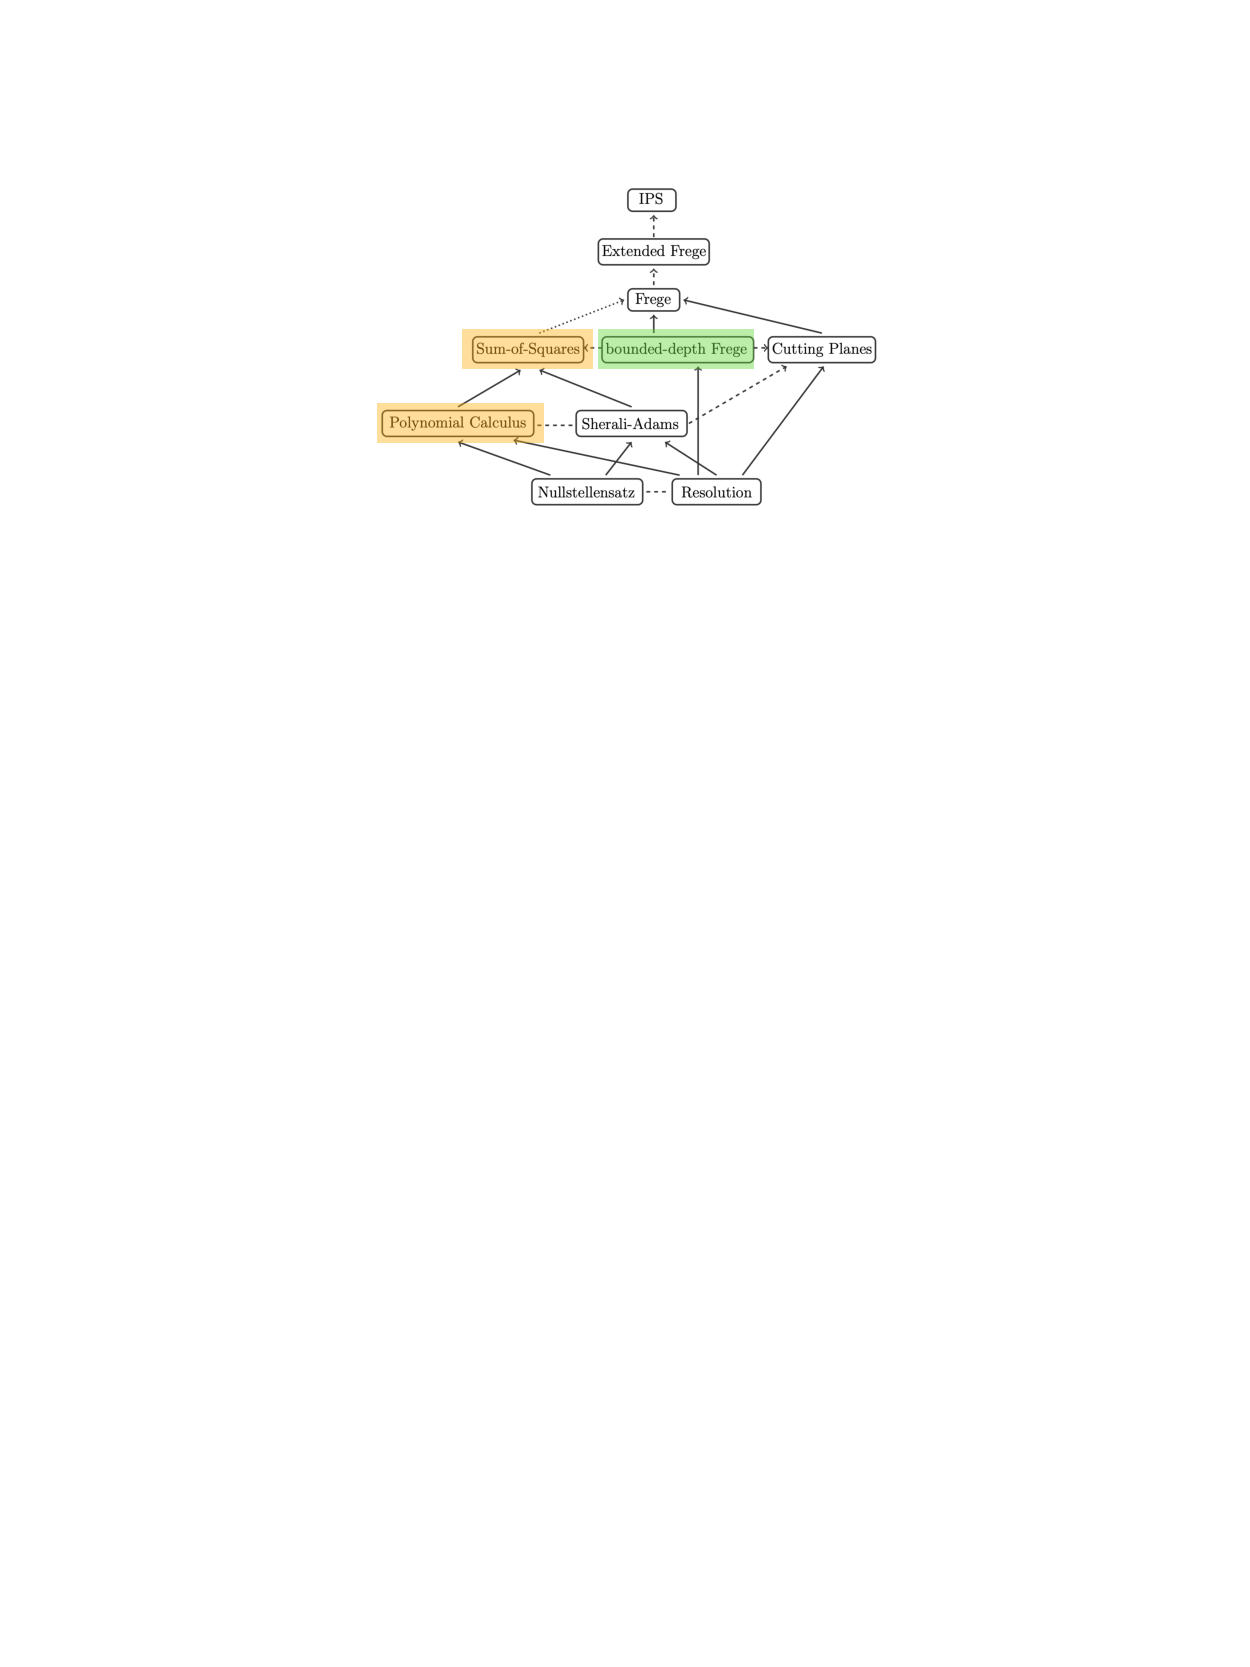
\includegraphics{assets/proof-system-relationships.pdf}
% 	\caption{The figure above (sourced from \citep[Page 9]{fleming2019semialgebraic}) depicts proof systems commonly studied by the community and how they relate to each other. We show lower bounds in the proof systems highlighted in orange, and as a consequence this also implies lower bounds in the bounded-depth Frege proof systems.}
% 	\label{fig:example-proof-systems}
% \end{figure}


Perhaps the most fundamental problem in computation is to provide an answer to the question asked by Cook and Reckchow in their seminal paper \citep{cook1979relative} -- ``\textit{Given a true statement $A$, is there a short proof of the claim that $A$ is true?}''
In trying to answer this question, we must first describe what constitutes a valid proof. That is, we must describe the language in which the proof is written (axioms), and the rules for checking it (the verifier).
Each set of rules for writing and checking a proof defines a proof system.
Therefore, a precise restatement of the question above is the following:  ``\textit{Given a true statement $A$ and a proof system $S$, what is the length of a shortest $\Proof \in S$ that proves $A$?}''
If we could show that there exists a proof system $S$, such that for \emph{any} true statement $A$, the length of the shortest proof in $S$ is upper bounded by some polynomial in the length of $A$, it would imply that $\CoNP = \NP$ and consequently $\P = \NP$. 
Conversely, if we could show large proof size lower bounds for some $A$ in \emph{all} proof systems, it would lead to a formal proof of the widely believed conjecture that $\P \neq \NP$.
Unfortunately, such lower  bounds for \emph{arbitrary} proof systems are out of reach.
As an intermediate step,
%towards making partial progress towards the grand problem, 
the research community has invested a significant effort in proving lower bounds for increasingly expressive proof systems (e.g.\ see \citep{abascal2021strongly, alekhnovich2001lower, atserias2020Size, buss1999linear,  conneryd2023graph, de2023clique, impagliazzo1999lower,  kothari2017SumOfSquares, potechin:LIPIcs.CCC.2020.38, raz2008elusive, razborov1998lower, schoenebeck2008linear}). \par
%Figure \ref{fig:example-proof-systems} lists some of these proof systems and describes the relationships between them.
 %Proof systems listed at the top of Figure \ref{fig:example-proof-systems} are more expressive\footnote{Expressiveness is formalised by the notion of $p$-simulation, and we refer the reader to \citep[Definition 1.6]{ProofComplexityLecNotes} for more details.}, and lower bounds for such proof systems subsume claims about the complexity of proofs lower in the figure.
%Thus, in an attempt to separate $\NP$ from $\CoNP$, the primary goal of proof complexity is to prove lower bounds for proof systems listed as high up in Figure \ref{fig:example-proof-systems} as possible.
% We refer the reader to \citep{krajicek2019proof, ProofComplexityLecNotesPaul} for more details. 
%these proof systems.
In this work, we focus on the algebraic and semi-algebraic proof systems of \emph{polynomial calculus (PC)} and \emph{sum of squares (SoS)}. %\citep{boazCourse,parrilo2000structured}.
In algebraic proof systems, we are given a set $\Axioms =\{\axiom_i(\vec{x}) \text{ } |\text{ } i \in [m] \}$ of $m$ polynomial equations\footnote{Semi-algebraic proof systems also allow for inequalities but we will not deal with inequality constraints in this paper.} over $n$ variables $\vec{x} = \{x_1, \dots, x_n\}$.
In PC, the coefficientcs can be over an arbitrary field $\Field$ and in the SoS the coefficients are  over the reals.
We say a proof $\Proof$ is a refutation of $\Axioms$, if it is a proof of the claim (in the specified language) that there exists no assignment of $\vec{x} \in \Field^n$ that satisfies \emph{all} the polynomial equations in $\Axioms$.
In PC and SoS, the proof $\Proof$ is itself expressed as a sequence of polynomials.
Two common measures of the complexity of the proof are the length of the sequence and the largest degree of the proof polynomials that refute $Q$ (see Section \ref{sec:proof-system-prelims} for more formal details).
Trade-offs between the two are well known; in particular, a lower bound on the degree implies a comparatively strong lower bound on the size of the proof.
Therefore, in this work we focus on the former. We denote the smallest maximum degree over all proofs that refute $\Axioms$ in PC and SoS, with $\Degree{Q \PC \bot}$ and $\Degree{Q \SOS \bot}$, respectively.
One motivation for proving lower bounds for algebraic proof systems, as opposed to propositional proof systems, is that often they imply lower bounds for a broad family of related algorithms for solving combinatorial optimisation problems.
Similarly, upper bounding the proof length has led to the fruitful discovery of many efficient algorithms.
The SoS proof system is of particular interest because of its close connection to the sum-of-squares hierarchy of semi-definite programming.
We refer the reader to the survey by Fleming, Kothari, and Pitassi \cite{fleming2019semialgebraic} for more details about the connections between the semi-algebraic proof systems and combinatorial optimisation.\par
In this work, we study the complexity of refuting \emph{perfect matchings} in PC and SoS.
Apart from being a natural problem in its own right, perfect matchings are also related to the pigeon hole principle \citep{maciel2000new, pitassi1993exponential, raz2004resolution, razbarov2002pgp, razborov2003resolution} and Tseitin formula \citep{filmus2013towards, galesi2019bounded, glinskih2017satisfiable, grigoriev2001linear}, two well studied formulae in proof complexity.
Assuming at most one pigeon fits in a single hole, the pigeon hole principle says $m$ pigeons cannot fit in $n < m$ holes.
If we construct the complete bipartite graph with the left vertices as $m$ pigeons and the right vertices as $n < m$ holes, proving the pigeon hole principle amounts to proving that such bipartite graphs does not have a perfect matching.
There are other formulations of the pigeon hole principle (see the survey by Razborov \citep{razbarov2002pgp}), and almost all of them have short proofs in the sum of squares proof system.
In contrast, Tseitin formulae is known to require long proofs. The Tseitin formula over a graph claims that there is a subgraph for which every vertex has odd degree.
If a graph has a perfect matching, then the subgraph described by the matching ensures that every vertex has odd degree.
However, formally refuting Tseitin formulae for expander graphs with odd number of vertices, in the SoS proof system, requires degree linear in the number of vertices in the graph \cite{grigoriev2001linear}.
% The exact complexity of refuting the perfect matching principle for expander graphs, however, remains unknown.
Given its close connections to the pigeon-hole and Tseitin, and the different behaviour of the two formulae, it is natural to determine the complexity of refuting perfect matchings for non-bipartite graphs.
To refute perfect matchings in an algebraic proof system, we first need to specify combinatorial constraints as algebraic equalities. Given an undirected graph $G=(V,E)$, $V = \{1, \ldots, n\}$, and a vector $\vec{b} = (b_1, \ldots, b_{n}) \in \Field^{n}$,
% we denote with $\vec{b} = (b_1, \dots, b_{|V|})  \in \Field^{\Size{V}}$ the vector of all $b$'s vector with size $\Size{V}$.
we define $\Card{G, \vec{b}}$ as the following set of polynomial constraints over variables $x_e$ for $e \in E$:

\[
        \Card{G, \vec{b}}=
        \Bigger[10]\{\begin{array}{@{}cl}
                x_{\highlight{e}}(1 - x_{\highlight{e}}) = 0 & \text{ for every $\highlight{e} \in E$}\\[3mm]
                % \underset{u \in \Neighbourhood{E}{\highlight{v}}}{\sum x_{(u,\highlight{v})}}= b_{\highlight{v}} & \text{ for every $\highlight{v} \in V$} \\[3mm]
                \sum_{e \sim \highlight{v}} x_e = b_{\highlight{v}} & \text{ for every $\highlight{v} \in V$} \\[3mm]
        \end{array}
\]
For every $e \in E$, the equation $x_e(1 - x_e) = 0$ restricts the domain of the above variables to bits.
In plain words, $\Card{G, \vec{b}}$ denotes the claim that there exists a spanning subgraph $G' \subseteq G$ such that a vertex $v \in V(G)$ has $b_v$ edges incident to it in $G'$.
Note if there was an assignment of variables $(x_e)_{e \in E}$ that satisfies all equations in $\Card{G, \vec{1}}$, where $\vec{1} = (1, \ldots, 1) \in \Field^{n}$, it would imply that the graph $G$ has a perfect matching (given by the edges corresponding to variables with assignment 1).
Therefore, we define $\PM{G} := \Card{G, \vec{1}}$.
When $|V|$ is odd, $G$ trivially does not contain a perfect matching. How difficult is it to refute $\PM{G}$ in this case? In recent work, Austrin and Risse \cite{Austrin_2022} showed that refuting $\PM{G}$, in the Polynomial Calculus  and Sum-of-Squares system, in the case $G$ is a \emph{random $d$-regular graphs} with an odd number of vertices typically requires proofs with degree $\BigOmega{n/\log n}$.
% \begin{theorem}\label{thm:prev-thm}
% There is a constant $d_0 \in \Naturals$ such that for all $d \geq d_0$, the following holds \emph{asymptotically almost surely} over a random $d$-regular graph $G=(V,E)$ on $n$ vertices (where $n$ is odd) \[ \Degree{\Card{G, \vec{1}} \SOS \bot} = \BigOmega{\frac{n}{\log n}}\]
% \end{theorem}
% Although random $d$-regular graphs are expander graphs with high probability, their techniques rely strongly on the randomness of sampling, and thus they are unable to extend their results to general expander graphs.
Their lower bound technique critically relies on the randomness of sampling, and therefore they can only only provide average case lower bounds.
They conjecture (see \citep[Section 6]{Austrin_2022}) that the hardness results should also apply to general expander graphs but leave showing so as an open problem.
In this work, we verify this by extending their result to all $d$-regular spectral expanders, that is, $d$-regular graphs with a mild condition on the spectral gap.
In fact, similar to Austrin and Risse, we reduce the hardness of refuting $\Card{G, \vec{t}}$, for any odd value $t$, to the hardness of refuting $\Card{G, \vec{1}}$.
As another special case, this answers the \emph{even-colouring} case $t = d/2$ is odd, a problem posed by Buss and Nordstr\"{o}m \citep[Open Problem 7.7]{buss2021proof}, which asks, \textit{``Are even colouring formulas over expander graphs hard for polynomial calculus over fields of characteristic distinct from 2 ?''}
Formally, we prove the following (for the definition of $(n, d, \lambda)$-graphs see Section \ref{sec:graph-theory-prelims}).


\begin{theorem}[Hardness Result For $\Card{G, \vec{t}}$]\label{thm:general-hardness-result}

  There exists universal constants $\epsilon, n_0, d_0 \in \Naturals$ such that for any odd $n \ge n_0$ and even $d \in [d_0, n]$, the following holds for \emph{any} $(n, d, \lambda)$-graph $G$ with $\lambda < \epsilon d$, and for any odd $1 \leq t \leq d$:  
  \[ \Degree{\Card{G, \vec{t}} \PC \bot} = \BigOmega{\nicefrac{n}{\log n}}\]
  \[ \Degree{\Card{G, \vec{t}} \SOS \bot} = \BigOmega{\nicefrac{n}{\log n}}\]  
\end{theorem}

\paragraph{Proof overview.}
We follow the overall approach of Austrin and Risse \cite{Austrin_2022}. Very briefly, the strategy is to obtain an affine restriction (see Definition \ref{def:affine-restriction}) $\Card{G, \vec{t}}|_\rho \equiv \PM{H}$ where $H$ is some graph for which refuting $\PM{H}$ requires large degree.
An example of such $H$ is given by Buss, Grigoriev, and Impagliazzo \cite{buss1999linear}. We now describe how to find such a restriction in more details: Using a result of Dragani\'c, Krivelevich, and Nenadov \cite{draganic22rolling}, we show that $H$ topologically embeds into a given expander graph $G$ with $\lambda \le \epsilon d$ for some universal small constant $\epsilon \in (0,1)$, such that all paths corresponding to the embedding have odd length.
The main technical ingredient of Austrin and Risse is also similar embedding theorem, but one that critically relies on the underlying graph being random.
As a random $d$-regular graph is with high probability an $(n, d, \lambda)$-graph with $\lambda = \Theta(\sqrt{d})$ (\cite[see Theorem A]{tikhomirov2016spectralgapdenserandom}), our embedding theorem subsumes that of \cite{Austrin_2022}.
Moreover, we show that one can find such an embedding so that the subgraph of $G$ induced by vertices which are not part of the embedding has a perfect matching.
This allows us to use the restriction argument to transfer the hardness of $\PM{H}$ into the hardness of $\PM{G}$.
To extend this to hardness of $\Card{G, \vec{t}}$ for an odd $3 \le t \leq d$, it suffices to show that the graph $G'$ obtained from $G$ by removing all edges that participate in the embedding and the matching contains a $(t-1)$-regular spanning subgraph.
Austrin and Risse achieve this using the contiguity property of random regular graphs; which naturally does not extend to arbitrary graphs.
Instead, we provide a significantly simpler and shorter, but more general argument based on Tutte's criterion.\par
The rest of the document as is structured as follows. In section \ref{sec:prelims}, we describe the requisite background from graph theory and proof complexity required.
In Section \ref{sec:embed-machinery}, we describe the machinery for finding a desired topological embedding.
In Section \ref{sec:matching-machinery}, we prove conditions under which the residual graph has a perfect matching or, more generally, a $(t-1)$-regular spaning subgraph.
In Section \ref{sec:main-proof}, we use the tools from the previous sections to prove Theorem \ref{thm:general-hardness-result}. 
In Section \ref{sec:related-work} we briefly discuss a few other lower bounds using embeddings in proof complexity, and then conclude with some future directions.

\section{Preliminaries}
\label{sec:prelims}


\subsection{Proof Complexity Preliminaries}
\label{sec:proof-system-prelims}

Let $\Axioms = \{ p_1 = 0, \dots, p_m = 0\}$ be a set of polynomial equations, which we refer to as axioms, over variables $\vec{X} = \{x_1, \dots, x_n, \bar{x}_1, \dots, \bar{x}_n\}$.
We will always assume that the axioms $x_i^2 - x_i = 0$ and $\bar{x}_i^2 - \bar{x}_i = 0$ are included in $\Axioms$ for all $i \in [m]$, which ensures that $x_i \in \bit$ for all $i\in [m]$.
Additionally, we will also assume that $1 - x_i - \bar{x}_i=0$ is also include for all $i \in [m]$, which ensures that the bar elements are bit complements of the non-bar elements.

\begin{definition}[Sum Of Squares Proofs]\label{def:sum-of-squares} Given a set of equality constraints $\Axioms$, a Sum of Squares (SoS) proof of $h \geq 0$ from $\Axioms$ is a set of polynomials $\Proof = (t_1, \dots, t_m; s_1, \dots, s_A)$ such that

\[ \sum_{i \in [m]} t_ip_i+ \sum_{i \in [a]} s_i^2 = h\]
The degree of a proof $\Proof$ is

\[ \Degree{\Proof} \Def \max\left\{\max_{i \in [m]} \Degree{t_i} + \Degree{p_i}, \max_{i \in [a]} 2\Degree{s_i}\right\}\]


\end{definition}


\begin{definition}[SoS Refutation]
An SoS refutation of $\Axioms$ is a proof of $-1 \geq 0$ derived from $\Axioms$. If we let $\Pi$ denote the set of all valid SoS refutations of $\Axioms$, then

\[ \Degree{\Axioms \SOS \bot} \Def \min_{\Proof \in \Pi}\Degree{\Proof}\]

\end{definition}

Polynomial Calculus (PC) is a dynamic version of the static Nullstellensatz proof system \citep[Section 1.3]{fleming2019semialgebraic} based on the following inference rules.
\begin{enumerate}
	\item From polynomials $f=0$ and $g=0$ where $f,g \in \Field[\vec{X}]$ we can derive $\alpha f + \beta g = 0$ for $\alpha, \beta \in \Field$.
	\item From polynomial $f=0$ where $f \in \Field[\vec{X}]$, we can derive $xf=0$ where $x \in \vec{X}$.
\end{enumerate}

\begin{definition}[Polynomial Calculus Refutations]\label{def:poly-calc-refutations}
A Polynomial Calculus (PC) refutation of $\Axioms$ over is a set of polynomials $\Proof = t_1, \dots, t_l$	such that $t_l = 1$, and for each $i \neq l$, either (1) $t_i \in \Axioms$, or (2) $t_i$ is derived from $\{t_j\}_{j < i}$ using the above rules.
The degree of the proof is given by $\Degree{\Proof} = \max_{i \in l}\Degree{t_i}$. If we let $\Pi$ denote the set of all PC refutations of $\Axioms$, then

\[ \Degree{\Axioms \PC \bot} \Def \min_{\Proof \in \Pi}\Degree{\Proof}\]
\end{definition}
Since we always assume the axioms contain constraints that restrict the variables to a boolean range by adding constraints $x_i^2 - x_i=0$ to the axioms, we can alternatively just work in the ring $\Field[x_1, \dots, \bar{x}_n]/(x_1^2 - x_1, \dots, \bar{x}_n^2 - \bar{x}_n)$ of multilinear polynomials.
Multi-linearity implies that the degree of any proof can be at most $n$ i.e a proof of degree $\BigOmega{n}$ is the largest lower bound one can hope to achieve.
The following lemma is by Buss, Grigoriev, and Impagliazzo \cite{buss1999linear} and gives an instance where perfect matching is hard to refute in the worst case. 

\begin{lemma}[Worst Case Hard Instance For PC]\label{lemma:worst-case-instance-PC}Given any odd $n \in \Naturals$, there exists a graph $H$ with $n$ vertices and maximum degree $\MaxDegree{H}= 5$ such that Polynomial Calculus over any field of characteristic different from 2 requires degree $\Theta(n)$ to refute $\Card{H, \vec{1}}$.
\end{lemma}
A description of the  worst case hard instance for SoS can be found in \citep[Theorem A.3]{Austrin_2022}.

\begin{lemma}[Worst Case Hard Instance For SOS]\label{lemma:worst-case-instance-sos}
Given any odd $n \in \Naturals$, there exists a graph $H$ with $n$ vertices and maximum degree $\MaxDegree{H}= 5$ such that SoS refutations requires degree $\Theta(n)$ to refute $\Card{H, \vec{1}}$.
\end{lemma}

\subsubsection{Affine restriction} 

An important lemma we will need is that given a set of axioms $\Axioms$ over the ring $\Field[x_1, \dots, x_n]$, a partial assignment of variables can only make refuting $\Axioms$ easier.
Given a set of $m$ polynomial equality constraints $\Axioms$ over boolean variables $\{x_1, \dots, x_n\}$, let the family of functions $\{f_i: \bit^n \rightarrow \{\True,\False\} \}_{i \in [m]}$, denote predicates for satisfiability for each constraint.
For example, given $\alpha \in \bit^n$, $f_i(\alpha) = \True$ if the $i$'th polynomial constraint $\axiom_i \in \Axioms$ is satisfied i.e $p_i(\alpha) = 0$.
We say $\Axioms$ is satisfied if $\exists \alpha \in \bit^n$ such that $f_i(\alpha) = \True \iff \axiom_i(\alpha)=0$ for all $i \in [m]$.
Given a map $\rho: \{x_1, \dots, x_n \} \rightarrow \{x_1, \dots, x_n, \bar{x}_1, \dots, \bar{x}_n, 1, 0 \}$, the restriction of a function $f: \bit^n \rightarrow \bit$, denoted by $f|_\rho$, is defined as $f|_\rho(x_1, \dots, x_n) = f(\rho(x_1), \dots, \rho(x_n))$.
Similarly, the restriction of formula $\Axioms$ is defined as $\Axioms|_\rho = \{f_{1}|_\rho, \dots, f_{m}|_\rho \}$.
Two formula $\Axioms$ and $\Axioms'$ are equivalent if they are element-wise equal, ignoring any functions that are constantly $\True$.
For example, $\Axioms = \{f_a, f_b, \True \}$ and $\Axioms' = \{f_a, f_b\}$ are equivalent, denoted as $\Axioms \equiv \Axioms'$.


\begin{definition}[Affine Restriction]\label{def:affine-restriction}
We say that an axiom $\Axioms'$ is an
affine restriction of $\Axioms$ if there is a map $\rho : \{x_1,\dots,x_n\} \rightarrow \{x_1, \dots, x_n, \bar{x}_1, \dots, \bar{x}_n, 1, 0 \}$ such that $\Axioms \equiv \Axioms|_{\rho}$.
\end{definition}


\begin{lemma}\label{lemma:affine_restriction}
Let $\Axioms, \Axioms'$ be axioms such that $\Axioms'$ is an affine restriction of $\Axioms$, and each axiom
of $\Axioms$ depends on a constant number of variables, then
\begin{enumerate}
	\item For any field $\Field$ it holds that $\Degree{\Axioms \PC \bot} \in \BigOmega{\Degree{\Axioms' \PC \bot}}$
	\item $\Degree{\Axioms \SOS \bot} \in \BigOmega{\Degree{\Axioms' \SOS \bot}}$
\end{enumerate}
\end{lemma}

The proof for the above lemma can be found in \citep[Lemma 2.2]{Austrin_2022}.
What the above lemma says is that if we have a graph $G$ with odd vertices woth constant degree, that has a perfect matching on a subset of even vertices on the graph, then the size of the proof to refute $\PM{G}$ is at least as large as refuting a perfect matching in $G$ with the even vertices removed.


\subsection{Graph Theory Preliminaries}
\label{sec:graph-theory-prelims}

We use standard graph theoretic notation. For a graph $\Graph$, we use $\Vertices{\Graph}$ and $\Edges{\Graph}$ to denote the vertices and edges of $\Graph$. For a vertex $v \in \Vertices{\Graph}$, we use $\Neighbourhood{G}{v} = \{ u \in \Vertices{\Graph} : (u,v) \in E' \}$ to denote the neighbourhood of $v$ in $G$, and $\degree{G}{v} := |\Neighbourhood{G}{v}|$. Given two sets $S, T \subseteq \Vertices{G}$, we  use $\CutEdges{S}{T}{G}$ to denote the number of edges in $G$ with one endpoint in $S$ and one endpoint in $T$.  Note that we do not require $S$ and $T$ to be disjoint; in case they are not disjoint, every edge with both endpoints in $S \cap T$ is counted twice in $\CutEdges{S}{T}{G}$. Given $W \subseteq V(G)$, we denote with $G[W]$ the subgraph of $G$ induced by $W$. We say that a subgraph $G' \subseteq G$ is \emph{spanning} if $V(G') = V(G)$.


% \rajko{I suggest the following notation: $e_G(S, T)$ denotes the number of edges with one endpoint in $S$ and the other in $T$. As we do not require $S$ and $T$ to be disjoint, any edge with both endpoints in $S \cap T$ is counted twice in $e_G(S, T)$. This is important as we use $e_G(S, S)$.}
% We assume the reader is familiar with standard graph theory definitions of subgraphs, minors, subdivisions and  topological minors.
% We refer the reader to \citep{bollobas2012graph} for a detailed introduction to these concepts.

Next, we give a definition of pseudorandom graphs.
% Throughout this paper, it suffices to treat $d$ as a constant.

\begin{definition}[$\EnDeeLambda$-graphs]\label{def:expander-graphs}
Let $G$ be a $d$-regular graph on $n$ vertices, and, let $\lambda_1 \geq \lambda_2, \dots, \geq \lambda_n$ denote eigenvalues of the adjacency matrix of $G$.
We say $G$ is an $\EnDeeLambda$-graph if $\ExpansionFactor{\Graph} := \underset{{\{2, \dots, n\}}}{\max}|\lambda_i| \leq \lambda$.
\end{definition}

The following is a well known result of Alon and Chung \cite{alon88mixing}.

\begin{lemma}[Expander Mixing Lemma]\label{lemma:expanders-mixing-lemma}
  Given an $\EnDeeLambda$-graph $G$ for any $S, T \subseteq \Vertices{G}$ we have
$$
  \left| \CutEdges{S}{T}{G} - \frac{d}{n}|S||T| \right|
  % \geq \frac{d\Size{S}\Size{T}}{n} - \lambda\sqrt{\Size{S}\Size{T} (1 - \frac{\Size{S}}{n}) (1 - \frac{\Size{T}}{n})   }	\\
  \le \lambda\sqrt{\Size{S}\Size{T} }
$$
\end{lemma}

% \begin{lemma}[Edge Connectivity In Pseudorandom Graphs]\label{lemma:edge-connectivity-pseudorandom}
% Every $\EnDeeLambda$ graph $G$ with $d - \lambda \geq 2$ has edge connectivity $\EdgeConnectivity{G} = d$.
% \end{lemma}
% \begin{proof}
%   We want to show that for all $S \subseteq \Vertices{G}$ of size $1 \leq \Size{S} \leq \frac{n}{2}$, we have $\CutEdges{S}{\Complement{S}}{\Edges{G}} \geq d$.
%   When $1\leq \Size{S} \leq d$, as $G$ is $d$ regular, every vertex in $S$ must have at least $d- \Size{S} + 1$ edges poking out poking out $S$.
%   Thus, the total edges out of $S$ is $\Size{S}(d- \Size{S} + 1)$ which has minimal value $d$.
%   If $d \leq \Size{S} \leq \frac{n}{2}$, use the tight version of the expander mixing lemma, and combined with the  fact that $d- \lambda > 2$ and $(n-\Size{S})$ is smallest when $\Size{S} = n/2$ to get the bound

%   \begin{align*}
%     \CutEdges{S}{\Complement{S}}{\Edges{G}} &\geq \frac{d\Size{S}(n-\Size{S})}{n} - \lambda\sqrt{\Size{S}(n-\Size{S}) (1 - \frac{\Size{S}}{n}) (1 - \frac{n-\Size{S}}{n})   }\\
%                                             &=  (d-\lambda)(\Size{S}\frac{(n-\Size{S})}{2}) \\
%                                               &\geq d
%     \end{align*}
  
% \end{proof}

% \begin{lemma}\label{lemma:d-connected-sets-have-no-bad-sets}
%   If $G$ has edge connectivity $\EdgeConnectivity{G} = d$, and $G$ is $d$-regular, then $\forall S \in \Vertices{G}$, $\OddComponents{G \setminus S} \leq |S|$.
% \end{lemma}
% \begin{proof}
%   As $G$ is $d$ regular, any set $S$ has at most $d\Size{S}$ edges incident on it.
%   By lemma \ref{lemma:edge-connectivity-pseudorandom}, as $\EdgeConnectivity{G} = d$, every component that connects to $S$ must have at least $d$ edges.
%   Therefore the maximum number of components we can have is $\Size{S}$.
% \end{proof}

We make use of the following two well known criteria of Tutte \cite{tutte1952factors, tutte1947factorization}.
Note that both of the lemmata ask for a property which is stronger than what Tutte criteria requires, though easier to state.
% The full proofs for \nameref{lemma:expanders-mixing-lemma} can be found in \citep[Theorem 2.11]{krivelevich2006pseudo}. Proofs for the \nameref{lemma:tutte-criterion} and \nameref{lemma:tutte-criterion-factor} can be found in \citep{genmatchings2025} and \citep{tutte1954short}, respectively. \rajko{Please cite the original work, not lecture notes.}

\begin{lemma}[Tutte's Criterion]\label{lemma:tutte-criterion}
Let $\OddComponents{G}$ denote the number of odd sized connected components in a graph $G=(V,E)$ with \emph{even} number of vertices. Suppose that for every $S \subseteq V$, $\OddComponents{G[V \setminus S]} \leq |S|$. Then $G$ contains a perfect matching.
\end{lemma}

\begin{lemma}[Tutte's Generalised Criterion]\label{lemma:tutte-criterion-factor}
  Let $\OddComponents{G}$ denote the number of odd sized connected components in a graph $G=(V,E)$ and $f \in \Naturals$ be even. Suppose that for every pair of disjoint sets $S, T \subseteq V$ the following holds:

  \[ |S|f \geq \OddComponents{S \cup T} + \sum_{w \in T} f - \Size{\Neighbourhood{E}{w} \setminus S}. \]
  Then $G$ contains a spanning subgraph $G' \subseteq G$ which if $f$-regular.
\end{lemma}



\subsection{Probabilistic Tools}

The proof of \nameref{lemma:mult-chernoff} and \nameref{lemma:lll}
can be found in any textbook on randomised algorithms \citep[See Chapter 1, Chapter 7]{mitzenmacher2017probability}.

\begin{lemma}[Multiplicative Chernoff bound]\label{lemma:mult-chernoff}
Suppose $X_1, ..., X_n$ are identical independent random variables taking values in $\{0, 1\}$. Let $X$ denote their sum and let $\mu = n\Mean{}{X_1}$ denote the sum's expected value. Then for any $0 < \delta < 1$

\[ \Prob{|X - \mu| \geq \delta \mu} \leq 2\exp(-\delta^2\mu/3)\]

\end{lemma}


A dependency graph for a set of events $E_1, . . . , E_n$ is a graph $G=(V, E)$ such that $V = \{1,.. . , n\}$ and,  for $i= 1,\dots, n$, event $E_i$ is mutually independent
of the events $\{E_j | (i, j) \notin E\}$. The degree of the dependency graph is the maximum degree of any vertex in the graph.


\begin{lemma}[Lov\`asz Local Lemma]\label{lemma:lll}Let $\Dist \in \DistSet{\bit^*}$ be a discrete probability distribution over bit strings of finite length.
  Let $E_1,...,E_n$ be a set of events, and assume that the following hold:
\begin{enumerate}
\item The degree of the dependency graph given by $(E_1, \dots, E_n)$ is bounded by $d$.

\item For all $i \in [n]$, $\PProb{E_i}{\Dist} \leq \beta$

\item $\beta \leq \frac{1}{4d}$.
\end{enumerate}
Then
\[ \PProb{\overset{n}{ \underset{i=1}{\cap}} \hspace{0.1cm}  \overline{E_i}}{\Dist} > 0\]


\end{lemma}

% Next we describe what it means to have a balanced cut of $G$.

% \begin{figure*}
%     \centering
%     \begin{subfigure}[t]{0.45\textwidth}
%         \centering
%         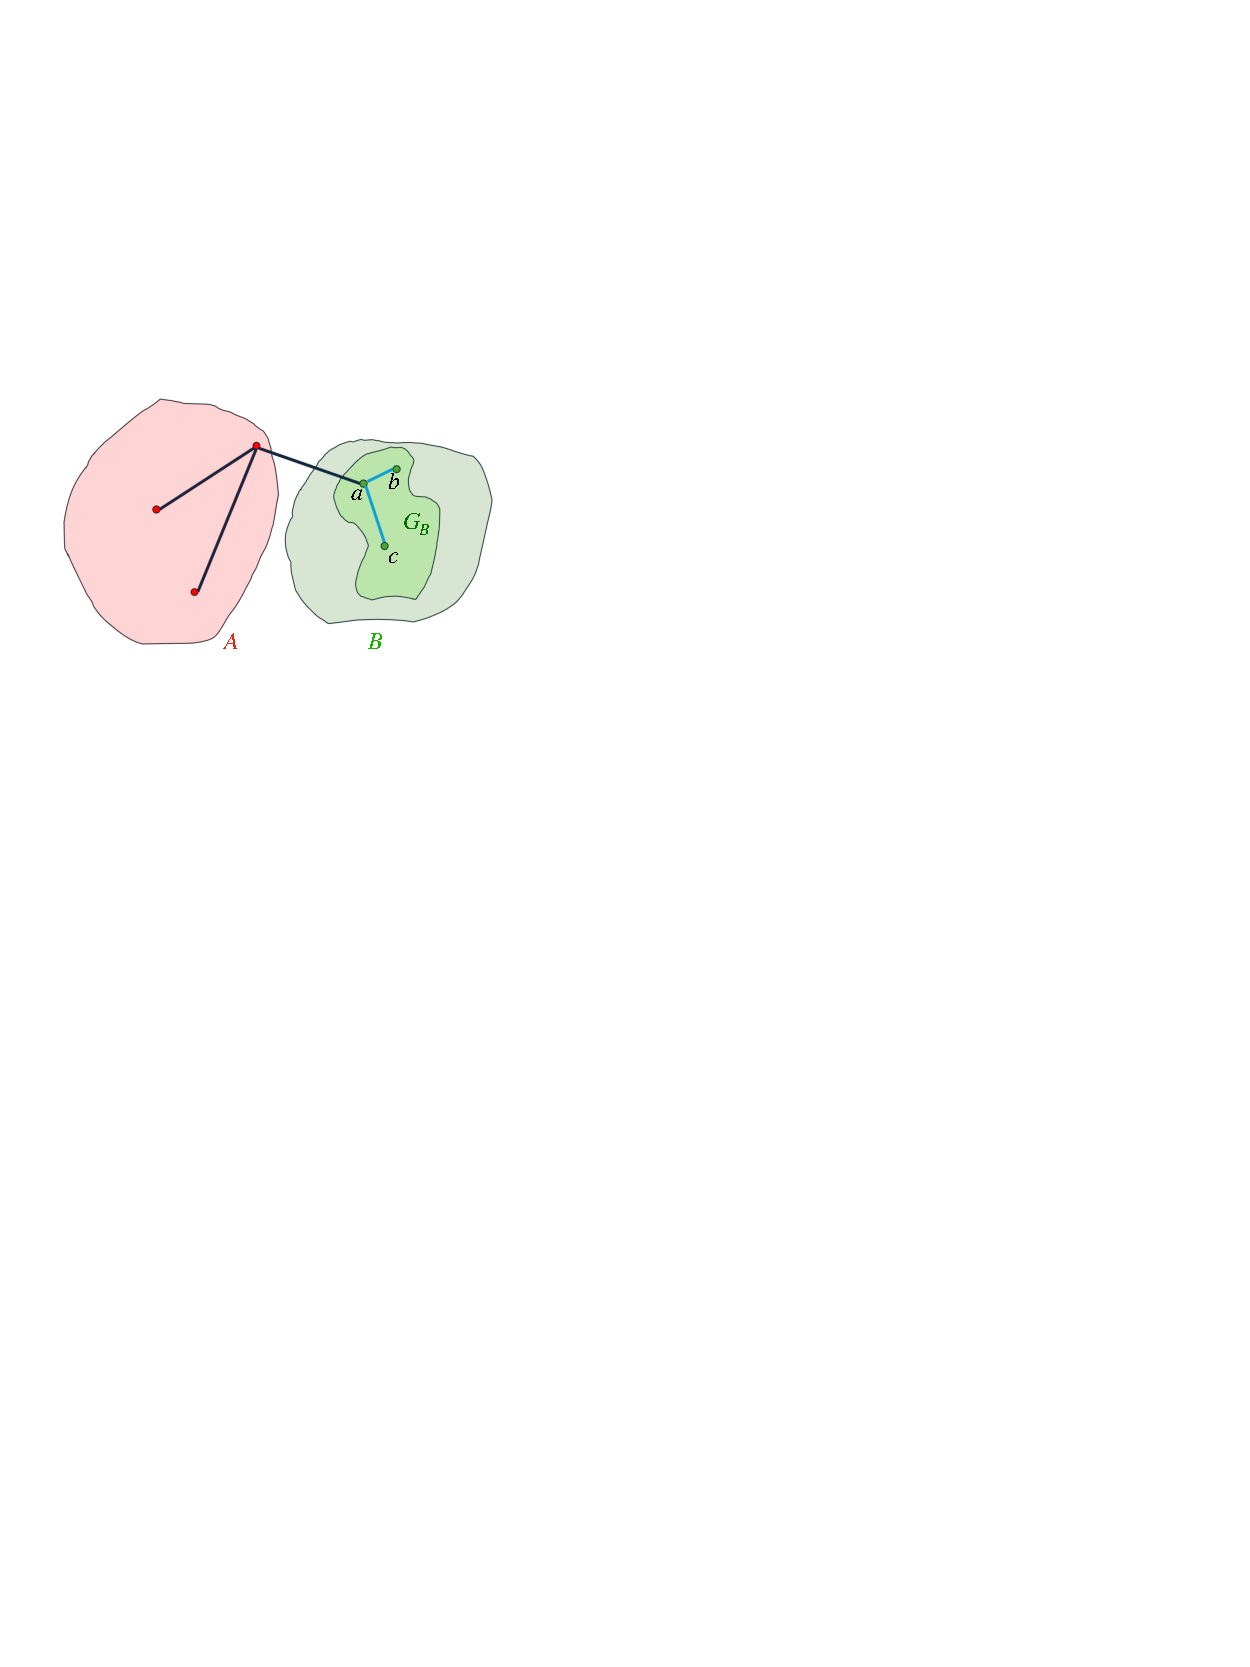
\includegraphics[width=\textwidth]{assets/partition-a.pdf}
%         \caption{}
%       \label{fig:partition}
%     \end{subfigure}%
%     \hspace{1mm}
%     \hspace{1mm}
%     \begin{subfigure}[t]{0.45\textwidth}
%         \centering
%         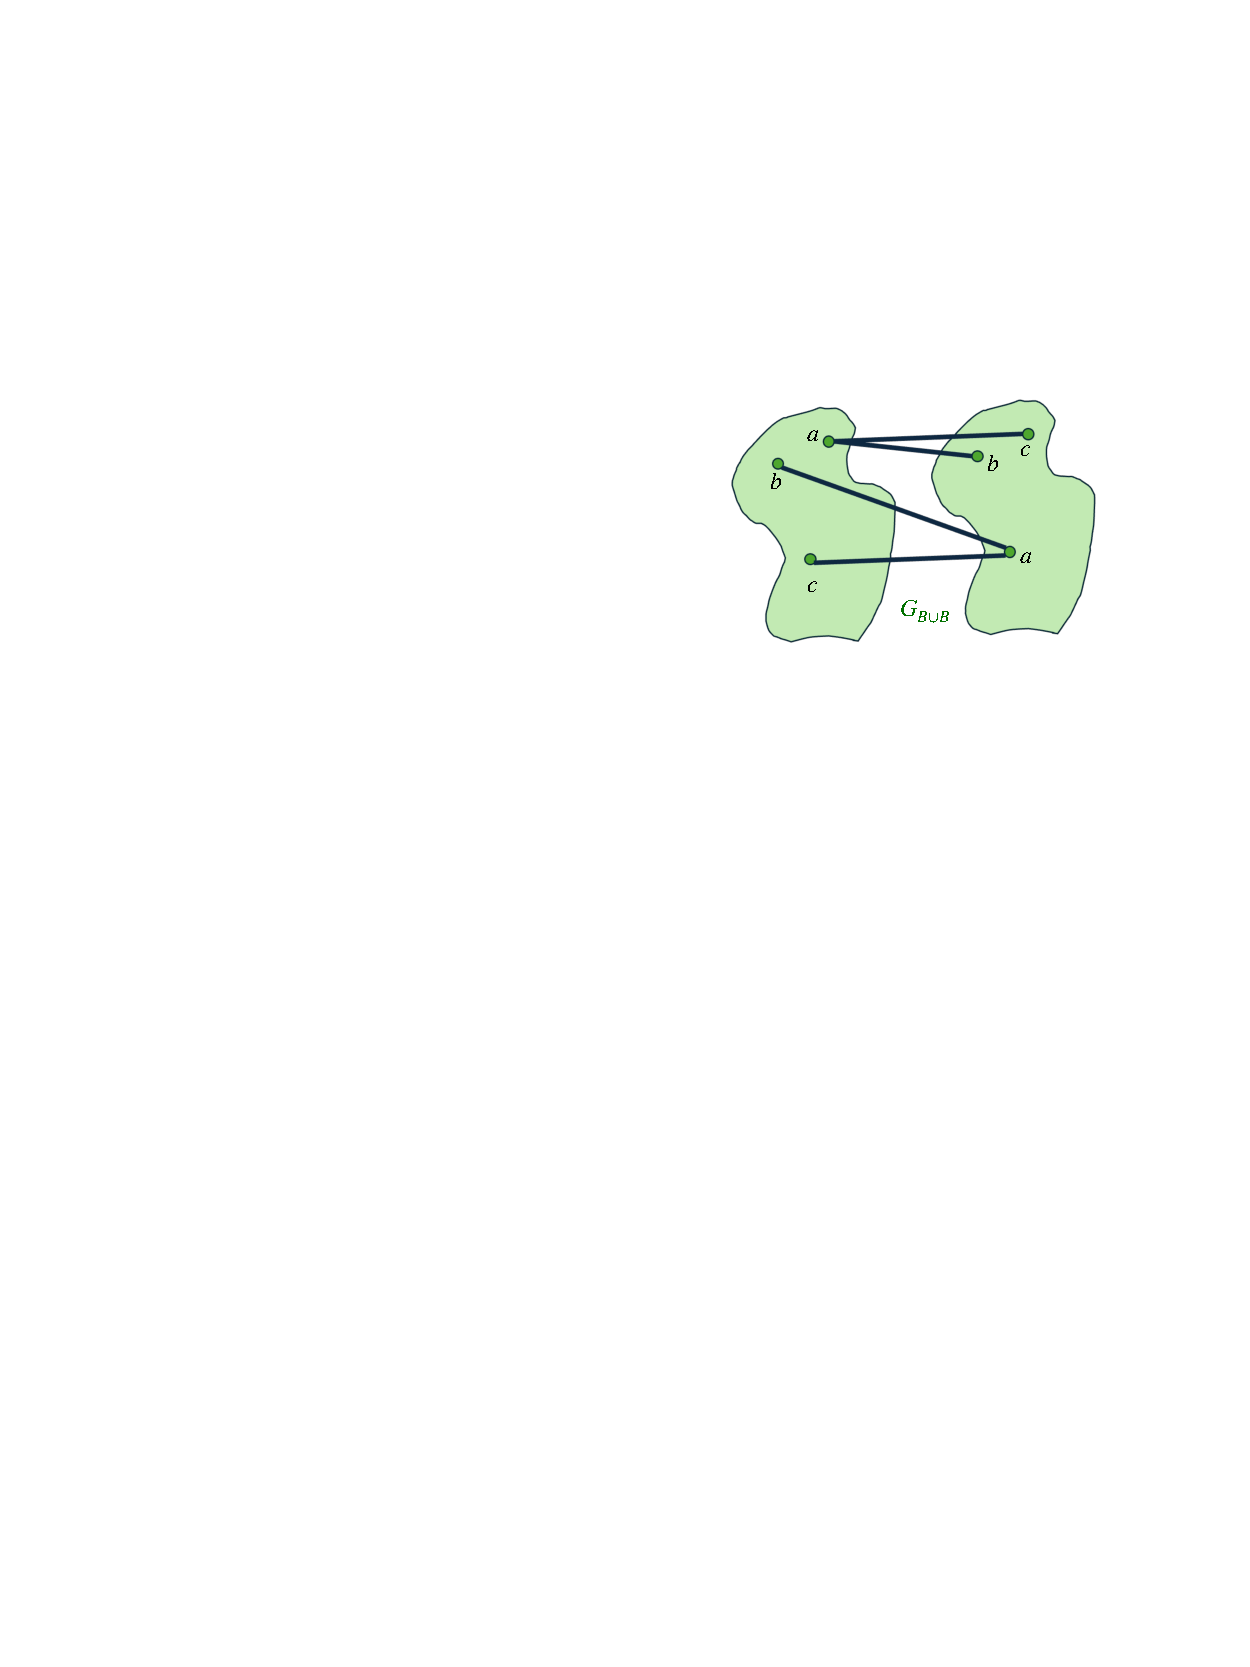
\includegraphics[width=\textwidth]{assets/partition-b.pdf}
%         \caption{}
%       \label{fig:bipartite}
%     \end{subfigure}
%     \caption{\small The figure above describes the partitioning of the vertices of the graph $G$ into two sets $\RedA$ and $\GreenB$, such that for every vertex $v \in \Vertices{G}$ has at least $11d/16$ \red{red} neighbours and at most $13d/16$ \red{red} neighbours. The subgraph $G_{\GreenB}$ obtained by including vertices in $\GreenB$ and edges that stay inside $\GreenB$. The figure on the right, depicts how the subgraph $G_{\GreenB}$ can be expressed as a bipartite graph $\BipartiteG$.}
%     \hspace{1mm}
% \end{figure*}


% \begin{definition}[Balanced Cuts]\label{defn:balanced-cuts} Given universal constants $0 \leq c \leq 1$ and $\epsilon > 0$, a $(c, \epsilon)$-degree balanced cut of a graph $G$ is a partition $\RedA \cup \GreenB$ of the vertices of $G$, such that, for every vertex $u \in \Vertices{G}$,  $cd - \epsilon d \leq \Neighbourhood{E}{u} \cap \RedA \leq cd + \epsilon d $
% \end{definition}

The following is the main result of this section.

\begin{lemma} \label{thm:partition}
For every $0 < c < 1$, and $\epsilon > 0$, there exists a constant $d_0 \in \BigOTilde{c/\epsilon^2}$, such that the following holds. If $G$ is a $d$-regular graph, for some $d \ge d_0$, then there exists a subset $A \subseteq V(G)$ such that
$$
    cd - \epsilon d \leq \left| \Neighbourhood{E}{v} \cap A \right| \leq cd + \epsilon d 
$$
for every $v \in V(G)$.
% on $n$ vertices, with $d \in [d_0, n-1]$, there exists and a  sets $\red{A}$ and $\green{B}$ is a $(c, \epsilon)$ balanced cut of $G$.
\end{lemma}
\begin{proof}
We prove the existence of such a partition $A \subseteq V(G)$ using the probabilistic method.
% We refer to elements in $\RedA$ as red nodes, and elements in $\GreenB$ as green nodes.
For each $v \in \Vertices{\Graph}$, we toss an independent coin $X_i$ with bias $c$.
If $X_i = 1$, then we include $v$ in $A$. Thus, $\vec{X} \Def (X_1, \dots, X_n) \in \bit^n$ is a random variable that describes how we choose $A$. For any $v \in V$, let $Y_v \Def |\Neighbourhood{E}{v} \cap \RedA|$ denote the random variable that counts the number of neighbours of $v$ in $A$.
Define $\delta \Def \epsilon / c$, and for every $v \in V$ let $E_v = \Indicator{|Y_v - d c | \geq \delta c d}$ denote the bad event that $v$ has too many or too few neighbours in $A$.
Observe that the dependency graph of events $\{ E_v \}_{v \in V}$ has maximum degree at most $d^2$ (only vertices at most two hops away from $v$ affect the colours of $v$'s neighbours; there at most $d^2$ such vertices).
% To see why, for any node $v$, let $u$ and $w$ denote vertices exactly 2 hops\footnote{A node $a$ is $k$ hops away from another node $b$ if the shortest path between $a$ and $b$ has $k$ edges.} and at least 3 hops away from $v$ respectively. The colour of $u$'s neighbours, directly affects how many red neighbours $v$ can have.
% However, as the colours for each node is sampled independently, the colour of $w$ or its neighbours do not affect $v$'s neighbours.
% Therefore $E_v$ is independent of $E_w$.
% There are at most $d^2$ nodes at a distance of at most 2 from any node, giving us the max-degree of the dependency graph.
As $\Graph$ is $d$-regular, $\Mean{\vec{X}}{Y_v} = c d$. By the \nameref{lemma:mult-chernoff}, for any $v \in V$ we have $\PProb{E_v}{\vec{X}} \leq 2\exp(-\delta^2c d/3) =: \beta$.
For $d_0 \in \BigOTilde{c/\epsilon^2}$ and $d \ge d_0$, we have $\beta \leq 1/(4d^2)$.
Therefore, $\beta d^2 \leq 1/4$. All the conditions of \nameref{lemma:lll} satisfied, from which we conclude that, with positive probability, none of the bad events happen. This implies the desired $A \subseteq V(G)$ exists.
% to get $\PProb{\underset{{v\in V}}{\land}\Complement{E_v}}{\vec{X}} > 0$.
\end{proof}


%We are given a pseudorandom graph $G$ on an odd number of vertices for $n$ large enough, and we want to show that refuting perfect matchings in the PC and SoS proof system requires large proofs.
%As described earlier, we do this by topologically embedding the above hard instance $H$ into $G$ while preserving the hardness of the original instance.

% \begin{remark}
%   \label{remark:edge-dist}
% For this section, and the next, we invoke Lemma \ref{thm:partition} with parameters. $c=3/4$ and $\epsilon=1/16$.
% Reviewing the properties of a balanced sets with $c=3/4$ and $\epsilon=1/16$, we have that every vertex $u$ in any $\EnDeeLambda$ graph  $G=(V,E)$,


% \end{remark}

\section{Topological embedding}
\label{sec:embed-machinery}

In this section we describe our first main ingredient, the topological embedding result of Dragani\'c, Krivelevich, and Nenadov \cite{draganic22rolling}. We start with a necessary definition.

\begin{definition}[Sub-divisions]\label{def:subdivisions}
Given a graph $H$ and a function $\sigma: \Edges{H} \rightarrow \Naturals$, the $\sigma$-subdivision of $H$, denoted by $\Subdivision{H}{\sigma}$, is the graph obtained by replacing each edge in $\Edges{H}$ with a path of length $\sigma(e)$ joining the end points of $e$ such that all these paths are mutually vertex disjoint, except at the end points.
\end{definition}

If a graph $G$ contains $H^{\sigma}$ for some $\sigma: \Edges{H} \to \Naturals$, then we say $G$ contains $H$ as a \emph{topological minor}. In our application, it will be important that we can control the parity of $\sigma(e)$. The following result follows directly from \cite[Theorem 1]{draganic22rolling}. 

\begin{theorem}[Embedding Theorem] \label{thm:embedding_top}
For every $D \in \mathbb{N}$ there exist $\alpha, \xi, C > 0$, such that the following holds. Suppose $G$ is a graph with $n$ vertices and $m \ge Cn$ edges such that for every pair of disjoint subsets $X, Y \subseteq V(G)$ of size $|S|, |T| \ge \xi n$, we have
$$
    \bigl| e_{G}(S, T) - |S||T|p \bigr| \le \xi |S||T| p, 
$$
where $p = m / \binom{n}{2}$. Then $G$ contains $H^{\sigma}$, where $H$ is any graph with maximum degree at most $D$, $H^\sigma$ has at most $\alpha n$ vertices, and $\sigma(e) \ge \log n$ for every $e \in E(H)$.
\end{theorem}

We make use of Theorem \ref{thm:embedding_top} through the following corollary.

\begin{corollary} \label{cor:embedding_top}
For every $D \in \mathbb{N}$ there exist $d_0, \epsilon > 0$, such that the following holds. Suppose $G$ is an $(n,d,\lambda)$-graph where $d \ge d_0$ and $\lambda < \epsilon d$. Let $B \subseteq V(G)$ be a subset of size $|B| \ge n/10$. Then the induced subgraph $G[B]$ contains $H^{\sigma}$, where $H$ is any graph with maximum degree at most $D$ and at most $\alpha n / (11 \log n)$ vertices, and $\sigma(e)$ is odd for every $e \in E(H)$.
\end{corollary}
\begin{proof}
    Let $m$ denote the number of edges in the induced subgraph $G[B]$. Then $2m = e_G(B, B)$, thus by \nameref{lemma:expanders-mixing-lemma} we have
    $$
        \left| 2m - \frac{d}{n}|B|^2 \right| \le \lambda |B|.
    $$
    Setting $p = m / \binom{|B|}{2}$, we have
    $$
        \left| p - \frac{d}{n} \right| \le 2 \lambda / |B|,
    $$
    with room to spare. Therefore, for every $S, T \subseteq B$ of size $|S|,|T| \ge \xi n$, for $\lambda < \epsilon d$ where $\epsilon$ is sufficiently small, we have
    \begin{align*}
        \Bigl| e_G(S, T) - p|S||T| \Bigr| &\le \left| e_G(S, T) - \frac{d}{n}|S||T| \right| + \left| \frac{d}{n}|S||T| - p|S||T| \right| \\
        &\le \lambda \sqrt{|S||T|} + 2 \lambda |S||T| / |B| \le \xi |S||T|p. 
    \end{align*}
    \rajko{Feel free to expand the previous calculation and explain it in more detail.}
    
    Let $\sigma: E(H) \to \Naturals$ be the constant function where $\sigma(e)$ is the smallest odd integer larger than $\log n$. Note that $\sigma(e) \le 2 + \log n$, thus $H^\sigma$ has at most $\alpha n / 10 \le \alpha |B|$ vertices. Therefore, we can invoke \nameref{thm:embedding_top} to conclude that $G[B]$ contains $H^\sigma$.
\end{proof}

\section{Perfect matching and regular subgraphs}
\label{sec:matching-machinery}
% Next we prove a lemma that shows that even sized subsets of expander graph with large minimal degree contain perfect matchings.
% has two parts.
% The first is an embedding theorem that allows us to transfer hardness of a worst case instance.
As described earlier, the second ingredient in our hardness proof is showing that a certain residual graph contains a perfect matching or a spanning $(t-1)$-regular subgraph. In this section we state and prove these ingredients.

\begin{lemma}[Perfect Matching Lemma]\label{thm:perfect-matching}
Suppose $G$ is an $(n, d, \lambda)$-graph, where $\lambda < d/50$. If $U \subseteq V(G)$ is of even size and $\delta(G[U]) \ge 11d/16$, then $G[U]$ satisfies the property of \nameref{lemma:tutte-criterion}. Consequently, $G[U]$ contains a perfect matching. 
\end{lemma}

\begin{proof}
  Suppose $U \subseteq V(G)$ is of even size and $\delta(G[U]) \ge 11d/16$.
  We show that $G[U]$ satisfies the property of \nameref{lemma:tutte-criterion}. Consider some $S \subseteq U$. We aim to show that $G[U \setminus S]$ has at most $|S|$ connected components (note that this is a stronger property than required). If $|S| \ge |U|/2$ then this trivially holds, thus we can assume $|S| < |U|/2$.
  It suffices to show that for every partition $X \cup Y$ of $U \setminus S$ such that $|X|, |Y| \ge |S|/3$, there exists an edge between $X$ and $Y$.
  Indeed, suppose that this holds but $G[U \setminus S]$ has more than $|S|$ connected components, with vertex sets denoted by $C_1, \ldots, C_k$, for some $k > |S|$.
  Then there is no edge between $X := C_1 \cup \ldots \cup C_{s}$ and $Y := C_{s+1} \cup \ldots \cup C_{k}$, where $s = \lfloor |S|/2 \rfloor \ge |S|/3$. As $|X|, |Y| \ge |S|/3$, we get a contradiction.

    Consider some partition $X \cup Y$ of $U \setminus S$ with $|X| \le |Y|$. Then $|X| \le (|U| - |S|)/2 \le (n - |S|)/2$. We show
    \begin{equation} \label{eq:edge_bound}
        \CutEdges{X}{X}{G} + \CutEdges{X}{S}{G} < \frac{11d}{16}|X|,
    \end{equation}
    as then the minimum degree assumption on $G[U]$ implies there has to be an edge with one endpoint in $X$ and the other in $U \setminus (X \cup S) = Y$. By the Expander Mixing Lemma we have
    \[
        \CutEdges{X}{X}{G} + \CutEdges{X}{S}{G} \le \frac{d}{n}|X|^2 + \lambda |X| + \frac{d}{n}|X||S| + \lambda\sqrt{|X||S|}.
    \]
    Using $|S|/3 \le |X| \le (n-|S|)/2$, $|S| \le n/2$, and $\lambda < d/24$,  we further upper bound the right hand side:
    \[
        \frac{d}{n} |X| \frac{n-|S|}{2} + \lambda |X| + \frac{d}{n}|X||S| + \lambda\sqrt{3} |X| < \frac{d}{2}|X| + \frac{d}{n}|X||S| + 3 \lambda |X| \le \frac{d}{4} |X| + 3\lambda |X| < \frac{11d}{16}|X|.
    \]
    This confirms \eqref{eq:edge_bound}. \rajko{Feel free to expand calculations, similarly how you did it in the next lemma.}
\end{proof}

\begin{lemma}[Regular Subgraph Lemma]\label{lemma:f-factor}
  Fix universal constant $C > 0$ and $d \ge d_0(C)$.
Suppose $G$ is an $\EnDeeLambda$ graph with $\lambda < \epsilon d$, where $\epsilon < 1/100C^{3/2}$.
If $G' \subseteq G$ has minimum degree $\MinimalDegree{G'} \ge d - C$, then $G'$ contains an spanning $f$-regular subgraph for any even $2 \le f \le d/2$.
\end{lemma}

\begin{proof}
  We prove this lemma using the \nameref{lemma:tutte-criterion-factor}.
  We need to show that for any pair of disjoint sets $S, T \subseteq \Vertices{G'}$
  \begin{align}
\OddComponents{S \cup T} &\le \Size{S}f - \sum_{w \in T} f - \Size{\Neighbourhood{E'}{w} \setminus S}
  \end{align}

As $G$ is an $\EnDeeLambda$ graph with $\lambda < \epsilon d < d/50$ and $G'$ has minimal degree $\MinimalDegree{G'} \ge d - C >  11d/16$, by the Lemma above, $G$' satisfies the strong \nameref{lemma:tutte-criterion} i.e. $\OddComponents{S \cup T} \le \Size{S \cup T} = |S| + |T|$.
  Thus, it suffices to show
  \begin{align}
    |S| + |T| &\le |S|f - \sum_{w \in T} f - \Size{\Neighbourhood{E'}{w} \setminus S}   \\
              &=\Size{S}f - \Size{T}f + \Size{T}(d-C) - \CutEdges{S}{T}{G'}  \label{eq:to-show}
  \end{align}  

  \textbf{Case 1}: If $\Size{S} \leq \Size{T}$, and as $f \leq d/2$, we have 
  \begin{align}
    \Size{S}f + \Size{T}(d-C-f)  &\ge (\Size{S} + \Size{T})(d/2 -C) \label{eq:to-show-1}
  \end{align}

\begin{align}
  |S| + |T| + \CutEdges{S}{T}{G'} &\le  |S| + |T| + |S||T|\frac{d}{n} + \epsilon d \sqrt{\Size{S}\Size{T}} \label{eq:eml}\\
                                 &\le |S| + |T| + \frac{d}{4}(\Size{S} + \Size{T}) + \epsilon d \frac{1}{2}(\Size{S} + \Size{T}) \label{eq:algebra}\\
                                 &\le (\Size{S} + \Size{T})\left(\frac{d}{4} + 1 + \frac{
                                   \epsilon d}{2}\right) \\
                                 &<  (\Size{S} + \Size{T})\left(d/2-C\right) \label{eq:eps-assumption}\\
                                 &\le \Size{S}f - \Size{T}(d-C-f) \label{eq:plug}
 \end{align}  
  
Equation \eqref{eq:eml} comes from the \nameref{lemma:expanders-mixing-lemma} and $\lambda < \epsilon d$.
Equation \eqref{eq:algebra} comes from the fact that $\Size{S}\Size{T} \leq \left(\frac{\Size{S}+\Size{T}}{2}\right)^2 \le n\frac{(\Size{S}+\Size{T})}{4}$.
Equation \eqref{eq:eps-assumption} comes from $\epsilon < \nicefrac{1}{100C^{3/2}}$.
Equation \eqref{eq:plug} follows from Equation \eqref{eq:to-show-1} which gives us what we want.

\textbf{Case 2}: If $\Size{S} > \Size{T}$, then 
  \begin{align}
    f\Size{S} +  \Size{T}(d-C-f)  &\ge 2\Size{S} +\Size{T}(d-C-2) \label{eq:to-show-2}
  \end{align}
  
  To show Equation \eqref{eq:to-show}, it suffices to show that
\begin{align}
  \CutEdges{S}{T}{G} \leq \Size{S} + \Size{T}(d-C-3) \label{eq:to-show-3}
\end{align}

Now we distinguish between two cases.

\begin{enumerate}

\item{
    If $\Size{T} \le \nicefrac{\Size{S}}{C+3}$, then we trivially have $\CutEdges{S}{T}{G'} \leq \Size{T}d$, and Equation \eqref{eq:to-show-3} follows from $\Size{S} \geq (C+3)\Size{T}$.
  }

\item{
$ \frac{\Size{S}}{C+3} < \Size{T} < \Size{S}$. As $\Size{S} + \Size{T} < n$, this assumption implies that $\Size{S} < n\left(1 - \frac{1}{C+3}\right)$.
Now using the \nameref{lemma:expanders-mixing-lemma}

\[ \CutEdges{S}{T}{G'} \le \frac{d}{n}\Size{S}\Size{T} + \epsilon d \sqrt{\Size{S}\Size{T}} \le \frac{(C-1)d}{D}\Size{T} + \epsilon d \Size{T}\sqrt{C} < \Size{T}(d-c)\]

which gives us Equation \eqref{eq:to-show-3}.
  }
  
\end{enumerate}
\end{proof}  



\section{Proof of Theorem \ref{thm:general-hardness-result}}
\label{sec:main-proof}

In this section we prove Theorem \ref{thm:general-hardness-result}. As $\Card{G, \vec{t}} \equiv \Card{G, \vec{d-t}}$, without loss of generality we only prove the theorem for $t \le d/2$. 

\begin{proof}[Proof of Theorem \ref{thm:general-hardness-result}]
Let $G=(V,E)$ be an $\EnDeeLambda$-graph on an odd number of vertices with $\lambda < \epsilon d$, where $\epsilon < \nicefrac{1}{100C^{3/2}}$ and $C=6$. Let $\HardInstance$ denote the graph on $h=\frac{n}{D \log n}$ vertices as given by Lemma \ref{lemma:worst-case-instance-sos} (to show lower bounds for PC, then we use $H$ from Lemma \ref{lemma:worst-case-instance-PC}). Recall that any SoS proof which refutes $\PM{H}$ has degree $\BigOmega{h}$. We now make use of $H$ to show the hardness of refuting $\Card{G, \vec{t}}$. The idea is to find a restriction $\rho$ such that $\Card{G, \vec{t}}|_\rho \equiv \PM{H}$. We achieve this through the following steps.

\begin{enumerate}
\item{Invoke Lemma  \ref{thm:partition} with parameters $c=3/4$ and $\epsilon = 1/16$ to get a subset $A \subseteq V(G)$ such that for every $v \in V(G)$ we have 
\begin{equation} \label{eq:size_nbr_A}
    \bigl| \Size{\Neighbourhood{G}{u} \cap A} - 3d/4 \bigr| \leq \epsilon d.
\end{equation}
This $|A| < n/2$, with room to spare. \rajko{Calculate the correct upper bound on $A$. If necessary, adjust the constant in Corollary \ref{cor:embedding_top}.}
}

\item{Let $B = V(G) \setminus A$. By Corollary \ref{cor:embedding_top}, $G[B]$ contains $H^{\sigma}$ such that each $\sigma(e)$ is odd. Let us denote a subgraph of $G[B]$ corresponding to $H^{\sigma}$ by $G_{\EmbeddingFunc}$. We can described $G_\EmbeddingFunc$ as a function $\EmbeddingFunc: V(H) \to B$ together with a collection of pairwise vertex-disjoint (other than at the endpoints) paths  $\Path{\Embedding{u}}{\Embedding{v}}$ in $G[B]$, for $(u,v) \in E(H)$.

    Observe that it is at least as hard to refute\footnote{Note that this by itself does not guarantee it is hard to refute $\PM{G}$. We need item (3) and this to show hardness in refuting $\PM{G}$.} $\PM{G_{\EmbeddingFunc}}$ as it is to refute $\PM{H}$.
    To see why, let $y_1, \dots, y_{E(H)}$ denote the variables for the $\PM{H}$ formulae for each edge of $H$.
    Let $\mathcal{Y} = (y_e)_{e \in E(H)}$ and $\Complement{\mathcal{Y}} = (\Complement{y_e})_{e \in E(H)}$. Define a mapping $\rho': \Edges{G_\EmbeddingFunc} \to \{0,1, \mathcal{Y}, \Complement{\mathcal{Y}} \}$ as follows. For each $(u,v) \in E(H)$, let $\rho'(x_e) = y_{u,v}$ where $e$ is the first edge on the path $\Path{\Embedding{u}}{\Embedding{v}}$. Map each variable $x_e$ for $e \in \Path{\Embedding{u}}{\Embedding{v}}$ alternately to $y_{u,v}$ or $\bar{y}_{u,v}$, such that the edges of the path adjacent to $\Embedding{u}$ and $\Embedding{v}$ are set to $y_{u,v}$. This is always possible as $\Path{u}{v}$ has odd length. Observe that $\PM{G_\EmbeddingFunc}|_{\rho'} \equiv \PM{H}$.
  }

\item{ As $n$ is odd and $\Size{\Vertices{G_{\EmbeddingFunc}}}$ is odd, we have that $U = \Vertices{G} \setminus \Vertices{G_{\EmbeddingFunc}}$ has even size. From \eqref{eq:size_nbr_A} we have that $G[U]$ has minimum degree at least $11d/16$. As $\lambda < d/50$, we can invoke the \nameref{thm:perfect-matching} to conclude $G[U]$ has a perfect matching $M$. 
}
  
\item{
  Consider the subgraph $G' \subseteq G$ obtained by deleting all edges $e \in \Edges{G_{\EmbeddingFunc}} \cup M$, where $M$ is the perfect matching from the step above. As $\MaxDegree{H} \leq 5$, every vertex $u \in G$ loses at most $5$ edges in this process. Thus, we have $\MinimalDegree{G'} \ge d - 5$. As $\lambda < \epsilon d$, by \nameref{lemma:f-factor} we have that $G$ contains a $(t-1)$-regular spanning subgraph $G'$. }

\end{enumerate}

We finally define $\rho$ as follows:
\[
\rho(x_e) =
\left\{
\begin{array}{@{}cl}
\rho'(e) & \text{if } e \in \Edges{G_{\EmbeddingFunc}} \\
1 & \text{if } e \in M \cup E(G') \\
0 & \text{otherwise}
\end{array}
\right.
\]
Then $\Card{G, \vec{t}}|_\rho \equiv \PM{H}$, thus our theorem follows from Lemma \ref{lemma:affine_restriction}.
\end{proof}


\section{Related Work And Concluding Remarks}
\label{sec:related-work}

\ari{I'm really not sure what else is actually related to our work. 
I could write about other results in proof complexity, but in that case we could just open the textbook on proof complexity and outline results. I fear we will be penalised for not having a bigger related work section, but at the same time there really isn't much more to talk about.
}
\rajko{I think it's fine. Leave it as is.}

In propositional\footnote{As opposed to algebraic proof complexity} proof complexity, there a few prior examples of the strategy of embedding a worst case instance into a host graph to show lower bounds for a larger class of objects \cite{itsykson2021Near, pitassi2016PolyLogFrege}.
Pitassi, Rossman, Servedio and Tan show Tseitin lower bounds for Frege proof systems \citep{pitassi2016PolyLogFrege} by relying on the embedding result by Rubinfeld and Kleinberg \citep{kleinberg1996short}, which allows one to embed any bounded degree graph $H$ of size $\BigO{n/\poly(\log n)}$ into an expander graph on $n$ vertices as a minor (not necessarily a topological one). 
Krivelevich and Nenadov simplify and improve the above embedding theorem to allow for embedding any graph $H$ with size $\BigO{n/\log n}$ as an ordinary minor \citep{krivelevich2021completeMinors}.
However, embedding a hard instance $H$ into $G$ as an ordinary minor does not guarantee that the hardness of $H$ is preserved.
It is entirely possible that one of the edge contractions to obtain the minor results in $H$ now being easy to refute.
Thus, these embedding theorems cannot be directly applied.
Instead, as described in section \ref{sec:main-proof}, one way to preserve hardness is to use  embedding theorems that allow for topological embeddings that allow for edge sub-divisions of odd size \citep{draganic22rolling, nenadov2023routing}.
In order to get a topological embedding, Austrin and Risse modify the ordinary embedding theorem in \citep{krivelevich2021completeMinors} but critically rely on the host graph being random.
In this work, we use the embedding theorem by Dragani\'c, Krivelevich, and Nenadov \cite{draganic22rolling}, which greatly simplifies the argument. Moreover, we avoid the use of the contiguity argument present in \cite{Austrin_2022} by directly utilising Tutte's criterion and the Expander Mixing Lemma.

\par
In summary, we show degree lower bounds for refuting $\Card{G, \vec{t}}$ for odd $t$ in $\EnDeeLambda$ graphs in the SoS and PC proof systems.
There is still $\log n$ gap between the largest possible proof in such systems, and our lower bounds (similar to Austrin and Risse).
It is not inherently clear that such a gap should exist.
This gap is predominantly an artefact of $d$ being constant, and using embedding theorems to prove hardness, as in exapnder graphs we  need $\Theta(\log n)$ edges to form a path between any two nodes.
This implies, that $\BigOmega{n/\log n}$ is the best we can do using embedding techniques.
Thus, if the worst case lower for refuting perfect matchings was indeed $\Omega(n)$, we would need a more direct proof of the statement using a different set of techniques.
We leave the issue of resolving the tightness of our lower bound as an open problem for future work.

% \newpage
\bibliographystyle{abbrv}
\bibliography{perfect-matching}
\clearpage
\appendix



\end{document}
